%% ----------------------------------------------------------------------------
% BIWI SA/MA thesis template
%
% Created 09/29/2006 by Andreas Ess
% Extended 13/02/2009 by Jan Lesniak - jlesniak@vision.ee.ethz.ch
%% ----------------------------------------------------------------------------
\documentclass[pdftex,11pt,openright,headsepline]{book}

\usepackage{paralist}		% List environment
\usepackage{color}		% For colored text
\usepackage{times}
\usepackage{amsfonts}		% Additional math fonts
\usepackage{amsmath}		% Math symbols
\usepackage{latexsym}
\usepackage{graphicx}		% For including images
% \usepackage{listings}		% If listings are needed
\usepackage{mydefs}		% Some of our own definitions
% \usepackage{wrapfig}		% To wrap images
% \usepackage{algorithmic}	% Nice algorithm environment
% \usepackage{algorithm}
\usepackage{fancyhdr}		% Produce the nice header
\usepackage{fullpage} % Use the full page
\usepackage{pdfpages}

\usepackage{amsmath}
\usepackage{hyperref}
\usepackage{algorithm}
\usepackage[noend]{algpseudocode}

\setlength{\headsep}{10mm} % gyglim: prevents from having text header

% Change the appearance of the header. Here \MakeUppercase is hard-coded, so renewing this command allows to elegantly change the header appearance.
\renewcommand{\MakeUppercase}{\scshape}

% Set the headings' appearance in the ``fancy'' pagestyle
\fancyhead{}
\fancyhead[RO, LE]{\leftmark}
\fancyfoot{}
\fancyfoot[RO, LE]{\thepage}

% The first pages shall be empty, even no page numbering


\begin{document}
\pagestyle{empty} % even no page number

\fancypagestyle{plain}{
  \renewcommand{\headrulewidth}{0.0pt}
  \fancyfoot{}
  \fancyhead{}
}

% Title page, modify accordingly
%% ----------------------------------------------------------------------------
% BIWI SA/MA thesis template
%
% Created 09/29/2006 by Andreas Ess
% Extended 13/02/2009 by Jan Lesniak - jlesniak@vision.ee.ethz.ch
%% ----------------------------------------------------------------------------

\begin{titlepage}

\thispagestyle{empty}

\fancypagestyle{empty}{
\lhead{\includegraphics[height=1.5cm]{images/ethlogo_black}}
\renewcommand{\headrulewidth}{0.0pt}
\rhead{\vspace*{-0.2cm}\includegraphics[height=1.4cm]{images/biwi_logo}}
\fancyfoot{}
}



\vspace*{2cm}
\begin{center}
\Huge{\textbf{My first and last thesis}\\}
\LARGE{\textbf{Subtitle Subtitle Subtitle}\\[1cm]}

\large{Master's Thesis\\[0.8cm]}
\LARGE{Eckhart Immerheiser\\}
\normalsize{Department of ....}
\end{center}

\begin{center}



% \begin{center}
% \begin{tabular}{ll}
% \multirow{2}{*}{\includegraphics[height=1cm]{images/biwi_logo}} & Computer Vision Laboratory\\
% & ETH Zurich
% \end{tabular}
%  \end{center}

\end{center}


\vfill
\begin{center}
\begin{tabular}{ll}
\Large{\textbf Advisor:} & \Large{Egon Hasenfratz-Schreier}\\
\Large{\textbf Supervisor:} & \Large{Prof.~Dr.~Luc van Gool}\\
% 			    & \small{Computer Vision Laboratory}\\
% 			    & \small{Department of Information Technology and Electrical Engineering}\\
\end{tabular}
\end{center}

\begin{center}
\today\\
\end{center}


\end{titlepage}

\cleardoublepage
%% ----------------------------------------------------------------------------
% BIWI SA/MA thesis template
%
% Created 09/29/2006 by Andreas Ess
% Extended 13/02/2009 by Jan Lesniak - jlesniak@vision.ee.ethz.ch
%% ----------------------------------------------------------------------------

\newpage
\vspace{3cm}

\chapter*{Abstract}
\noindent

Mobile devices with cameras now contain various photos ranging from natural
scenery and city skylines, to street signs and restaurant menus.
When deciding to review these various moments in daily life, one can opt to use
a wallpaper application which sets an image from the photo collection as a
wallpaper.
Unfortunately, not all photos are suitable nor well composed.
This study is a novel attempt to improve these aspects.
This is done by first deciding if an image is suitable to be used as a wallpaper,
and if so how it should be cropped and shown on a given display.
The selection algorithm yields a classification error as low as 3.7\% where images with annotations in agreement are evaluated.
The cropping algorithm is based on work by Fang et al. and yields an improved 0.782 median maximum overlap score, a $\sim6\%$ improvement.
Qualitative results are quite good where photos with less desirable objects are
omitted, and more interesting regions are retained in the final crops.


%% Input here any acknowledgements
%%% ----------------------------------------------------------------------------
% BIWI SA/MA thesis template
%
% Created 09/29/2006 by Andreas Ess
% Extended 13/02/2009 by Jan Lesniak - jlesniak@vision.ee.ethz.ch
%% ----------------------------------------------------------------------------


\newpage

\chapter*{Acknowledgements}


%\cleardoublepage
%\newpage

% % Chapter-pages etc. use the ``plain'' pagestyle - since we don't want to have a heading at all at chapter-pages, redefine plain accordingly. Don't forget the page number.
\fancypagestyle{plain}{
  \renewcommand{\headrulewidth}{0.0pt}
  \fancyfoot{}
  \fancyfoot[RO, LE]{\thepage}
  \fancyhead{}
}

\pagestyle{fancy}
\pagenumbering{Roman}

% Insert table of contents
\tableofcontents

% Insert list of figures
\listoffigures
\cleardoublepage

%% Insert list of tables
%\listoftables
%\cleardoublepage

\newpage

\pagenumbering{arabic}

%% ----------------------------------------------------------------------------
% Actual text comes here - defer it to other files and use \input{bla.tex}, ..
%% ----------------------------------------------------------------------------
%% ----------------------------------------------------------------------------
% BIWI SA/MA thesis template
%
% Created 09/29/2006 by Andreas Ess
% Extended 13/02/2009 by Jan Lesniak - jlesniak@vision.ee.ethz.ch
%% ----------------------------------------------------------------------------


\chapter{Introduction}

The widespread use of mobile computing devices such as smartphones and tablet
computers has led to the creation of large personal photo collections.
Unlike previous methods, photo capture using modern smartphones has a low cost.
There are low space restrictions and photos are simple to take with modern
applications.
This leads to lower inhibition in taking photos, and a wider variety photos in
less carefully curated collections.
These collections can include photos capturing among other objects:

\begin{itemize}
\item Natural scenes
\item Cityscapes
\item Quick notes (street signs, maps, documents)
\item Screenshots
\item Quick shots for instant messaging
\end{itemize}

It may sometimes be desirable to review some photos from a mobile phone via the use of widgets or wallpaper carousels.
One such application which serves this purpose is Muzei for Android \footnote{\url{http://www.muzei.co/}}.
A user can set Muzei to show a random photo from the mobile phone gallery as a wallpaper with a new photo being chosen at a set time interval.
It should be noted that such a photo carousel may suffer from two issues.

\begin{figure}
\centering
\begin{subfigure}{0.46\columnwidth}
  \centering
  \includegraphics[width=0.95\columnwidth]{../figures/Michael/2013-12-04 13.44.24.jpg}
  \caption{An academic poster, useful for review purposes but not possibly unsuitable as a wallpaper.}
\end{subfigure}
\hfill
\begin{subfigure}{0.46\columnwidth}
  \centering
  \includegraphics[width=0.95\columnwidth]{../figures/Michael/2013-12-25 16.32.32.jpg}
  \caption{Scene of a beach at a vacation destination. Possibly suitable as a wallpaper.}
\end{subfigure}
\caption{An example of a potentially suitable and unsuitable photo to use in creating a wallpaper for a mobile device.\label{fig:good_n_bad_wallpaper}}
\end{figure}

The first issue is that certain photos may not be suitable to be used as a wallpaper.
For instance, a bus route timetable may be useful to have for the cases where an estimated travel time is required, but not the most aesthetically pleasing image to have on the background of a mobile phone.
An example of this is illustrated in figure \ref{fig:good_n_bad_wallpaper}
At the most basic level, the objects present in the image could be used to determine if it would be suitable.

The second issue comes from the alignment or cropping of a photo.
Since a photo must be formatted appropriately to be shown on the given display, some information has to be discarded.
A naive approach of centering the photo may lead to the cutting or complete omittance of objects.
It would be desirable to crop a given image to a target aspect ratio without losing interesting regions.
To this effect, work from \ref{fang2014automatic} is expanded on to provide an effective automatic cropping algorithm.

This project aims to address the two mentioned issues: determination of wallpaper suitability and image cropping to fit a target display in an aesthetically pleasing manner.
In short form, we will refer to the two areas as \emph{Selection} and \emph{Cropping}.

To solve the photo selection problem, we propose a simple algorithm based on object class recognition and machine learning in section \ref{sec:meth_selection}.
Out of a collection of images which have been annotated by 4 individuals, a subset is selected where annotations have consensus.
The annotations are for whether the corresponding image should be used as a wallpaper.
The final selection algorithm performs well on this dataset with an error of just 3.7\%.

The cropping of images is carried out using a saliency and learning based model which derives from the algorithm introduced in \cite{fang2014automatic}.
We extend the algorithm by considering boundary simplicity conditions for each image edge and employing a shrinking heuristic for evaluating potential crop regions.
This work is outlined in section \ref{sec:method_cropping}.
Our algorithm outperforms the approach of \cite{fang2014automatic} by approximately 6\%, achieving a maximum overlap of $0.782 \pm 0.004$ with crop regions annotated by professionals via the Amazon Mechanical Turk platform.
The annotations are sourced from \cite{fang2014automatic}.

In the following sections, We introduce the methodology and used datasets for both wallpaper selection and automatic cropping, and evaluate the performance of the two algorithms in a quantitative and qualitative manner.


%% ----------------------------------------------------------------------------
% BIWI SA/MA thesis template
%
% Created 09/29/2006 by Andreas Ess
% Extended 13/02/2009 by Jan Lesniak - jlesniak@vision.ee.ethz.ch
%% ----------------------------------------------------------------------------
\newpage
\chapter{Related Work}

As mentioned in the previous section, the aim is to improve the experience of
viewing photos from a mobile phone gallery as wallpapers.
This requires the determination of whether an image should be selected for
display, and the selection of a window or crop of the original image which
should be displayed on a given screen.

There is no prior work for automatically selecting wallpapers.
The most similar work is the summarisation of photo albums
\cite{sinha2009personal}.
Unfortunately, there is lack of detail and reliance on detailed
annotations.
Thus in this study, the problem of deciding if a photo could be used as a
wallpaper is dealt with in a simple manner which requires minimal annotations.

Depending on which object or scene is given focus, an image can be perceived
very differently by a viewer.
Thefore there is great interest in attempting to improve how well an image is
composed.
To this effect, there have been many previous studies in cropping or deforming
images to a target size or aspect ratio.

Seam carving is an effective way to removing less
interesting seams or regions in an image but unfortunately can warp the image
badly when failing to work successfully \cite{avidan2007seam}.
Other similar methods such as Multi-operator retargeting also suffer from
heavy deformation and artifacts depending on the input image \cite{rubinstein2009multi}.
In fact, \cite{rubinstein2010comparative} notes that:
\emph{"Cropping, although a relatively naive operation, is still one of the most
	favored methods, most often since it does not create any artifacts. Our
	findings indicate that the search for an optimal cropping window, which
	was somewhat abandoned by researchers in the past few years, could often
	be favorable and should not be overlooked."}
Therefore, cropping algorithms are focused on for choosing how to display a
candidate wallpaper image on a given display.

The automatic cropping of an image can be done in two major ways, one which
requires a set of rules, and a learning-based model which associates a set of
features to a score.
Rules-based croppers such as \cite{liu2010optimizing, zhang2005auto} can suffer
from bias or imprecision due to human-selected rules and parameters.
Learning-based croppers such as \cite{park2012modeling, yan2013learning} are
not without fault however, with low precision due to lack of training data being
a particularly big issue.

A novel method suggested by Fang et al. \cite{fang2014automatic} attempts to
combine the advantages of both approaches by introducing three cues into the
learning and cropping stages.
These include saliency composition, boundary simplicity, and content
preservation.
This is described in greater detail in the next sections.
Another improvement in the suggested method is the use of public datasets such
as those which can be found on image hosting services such as Flickr and
Photo.net.
These services can indicate how good an image is perceived to be and allow for
automatic annotation of possible image crops.


%% ----------------------------------------------------------------------------
% BIWI SA/MA thesis template
%
% Created 09/29/2006 by Andreas Ess
% Extended 13/02/2009 by Jan Lesniak - jlesniak@vision.ee.ethz.ch
%% ----------------------------------------------------------------------------
\newpage
\chapter{Materials and Methods}

This project consists of two parts. When given a set of photos taken using a
mobile phone, the first part is the selection of photos and the second part is
the cropping of photos.
The selection criteria is wallpaper suitability while the cropping aims to
retain interesting areas to result in a well composed final image.

Both decisions are subjective by nature.
If a set of rules were defined to make the decisions, the process would
inherently be biased, and results difficult to evaluate.
Thus for both selection and cropping, machine learning is utilised with aims to
avoid introducing unnecessary bias.


\section{Selection\label{sec:meth_selection}}

When considering a single photo, whether this photo could be used as a wallpaper is a subjective decision.
Ultimately, the decision depends on whether a photo is aesthetically pleasing to view in the background of the home screen of a mobile device.
This may depend not only on the objects present in the scene, but image sharpness, colour composition, and density of detail.
At the most basic level, it can be argued that the most important factor is the objects present.
For instance, person A may prefer having city skylines on their wallpapers, while person B may prefer distant mountain peaks.
When considering objects which most people would not like to have on their wallpapers, we can think of posters, advertisements, and price tags as examples.
The detection of such objects would allow for a simple but effective way of picking or discarding images when attempting to find a suitable wallpaper.
We therefore suggest a simple algorithm which performs object class recognition to determine if an image is suitable as a wallpaper.

To address the inherent subjectivity of this process, we employ machine learning and acquire annotations from multiple individuals.
By doing so, it is possible to train a model such that it can cater to the preferences of all annotators as well as possible.
A feature vector is created per image, encoding information on detected objects.
These vectors can be used to train a SVM.

One way of performing object class recognition is via the use of deep
convolutional neural networks.
An existing implementation is one provided by Caffe, a deep learning framework\cite{jia2014caffe}.
Caffe provides several models trained for the ILSVRC 2012 dataset \cite{ILSVRC15}.
This dataset consists of 150,000 photographs and 1,000 associated object classes.

In a deep convolutional neural network, different convolutions are performed at
each neuron with a focus on different portions of a given image.
In \cite{DonahueJVHZTD13}, it is determined that using the activations of the
hidden fully connected layer, \texttt{fc7} in conjunction with a SVM results
yields the best classification results in domain adaptation tasks such as scene recognition.


Therefore, an input image is propagated through the trained neural network and
the activations at hidden layer \texttt{fc7} is used as the given image’s
representative feature vector.
The exact neural network used is \texttt{bvlc\_reference\_caffenet}.
This results in 4096 features per image.
These feature vectors are used to train a SVM.
The decision function of the trained model calculates a suitability score when
provided a feature vector representative of an input image.
If an image is classified as positive, it is considered to be suitable.

The resulting model can then be used to classify new images.
Figure \ref{fig:pipeline_selection} shows the full pipeline for
checking the suitability of an image as a wallpaper on a mobile device.

\begin{figure}
\centering\includegraphics[width=0.7\columnwidth]{../figures/pipeline_suitability.pdf}
\caption{Full pipeline for determining if an image is suitable for use as a wallpaper.\label{fig:pipeline_selection}}
\end{figure}

This portion of the project is implemented using \texttt{Python},
\texttt{scikit-learn}, \texttt{OpenCV}, and \texttt{PIL}.

\subsection{Datasets}

Two datasets were created for the selection step. I will call these datasets the
\emph Michael dataset and the \emph Wookie dataset.

The Michael and Wookie datasets consist of 275 and 266 images each respectively.
The photos image a variety of objects and scenes with some example objects
as listed below:

\begin{itemize}
\item Natural landscapes (Mountains, rivers)
\item Man-made landscapes (Cityscapes, landmarks)
\item Text (Poster, presentation, street sign)
\item Dim indoors (Concert, restaurant, presentation)
\end{itemize}

While the photo collections were created with aims to provide sufficient variety
to result in a more general purpose model, privacy was respected and thus the
datasets lack people.

The ground truth was collected by annotation from 4 different volunteers.
Each person was asked to mark images in both datasets as either suitable or
unsuitable (1 or 0 respectively) based on the simple rule: \emph{"rate as
suitable if you would personally use the image or a portion of the image as a
wallpaper on your phone"}.

In early annotations, it was evident that the order in which images was
displayed affected final decisions.
If similar images were shown in succession, the classifications could become
less consistent.
The order was therefore randomised.
A simple Python script was written to accommodate this effort.
Key bindings were added to allow for effortless annotation and navigation
between images, and the images are tinted green or red depending on the decision
to allow for quick review.

A further improvement could be made by splitting annotators into two groups, one
which make a preliminary set of annotations which can be used to create a
balanced dataset which is annotated by the other group of annotators.
This would reduce bias further.

\section{Cropping\label{sec:method_cropping}}

This study bases its cropping method on \cite{fang2014automatic} with modifications.
The differences are namely in moving boundary simplicity into the learning phase, the use of shrinking crop region candidates in crop selection, and the use of a Reddit based dataset.
This is further outlined below as the algorithm is explained.

To crop an image automatically, it should be possible to find out which regions
of the image are worth retaining.
To do so, we consider visual saliency.
Visual saliency is a measure which represents how distinct a region is in
relation to its neighbouring regions \cite{borji2013state}.
Many saliency map algorithms have been suggested in the past, with ground truth
collected by tracking the eye movements of human participants.

The algorithm selected for generating visual saliency maps is the boolean map
based approach or BMS \cite{zhang2013saliency}.
This approach randomly thresholds each channel in CIE Lab colour space to
generate a set of boolean maps, then averages the boolean maps to generate an
attention map.
The algorithm is very fast and produces high quality saliency maps.
The output saliency map is further dilated and blurred in an attempt to give
crop candidates a good margin from objects.

An input image is first scaled to be at most 800 pixels wide or high, then a
dilation width of $2$ pixels and step size of $6$ is used to generate an initial
saliency map.
This map is further processed with a dilation filter of width $5$ pixels and a
$11\times11$ gaussian blur filter with $\sigma=50$.

In \cite{fang2014automatic} automatic cropping is done using three distinct metrics.
These are saliency composition, boundary simplicity, and content preservation.
Saliency composition concerns the layout of saliency energy, and boundary
simplicity is whether the crop cuts through objects, while content preservation
is the proportion of saliency energy kept in the crop.
In our approach saliency composition and boundary simplicity are encoded into
the learning stage where an SVM is trained to distinguish between well and badly
composed images or crops.
The content preservation metric is used in the filtering of crop candidates in
the cropping stage.

Saliency composition is represented by a 4-level spatial pyramid of the saliency
map.
This is done by resizing the map into $8\times8$, $4\times4$, $2\times2$, and
$1\times1$ patches
by averaging pixel values, then using pixel values in these patches as features.
This results in 85 features which encode the distribution of saliency energy.

Boundary simplicity aims to encourage crops which do not cut through objects.
This can be done by taking a gradient map of the original image.
A 2-pixel wide strip is taken for each edge and the mean value is used as a
feature.
This results in 4 features encoding the amount of edges crossed by a given
crop's boundary.
This is different from the implementation in \cite{fang2014automatic} where a single boundary simplicity score is used later on in the evaluation of candidate crop regions.
We introduce these changes for two reasons.
The first is to avoid the weighting issue when dealing with multiple metrics in the final scoring of crop candidates, instead relying on SVM.
The second reason is to allow for boundary metric to adapt to cases where saliency composition may affect boundary values.
For example, a portrait photo of a person may have high saliency on the bottom edge of the image but still be considered to be well composed with good boundary simplicity.

The gradient map of an image is created by first resizing the image to be at
most 600 pixels wide or high, then applying a first-derivative $5\times5$ Sobel
filter.
Absolute values are taken per pixel, then a $11\times11$ Gaussian blur filter
($\sigma=50$) is applied.
This results in an image similar to the corresponding saliency map where object
boundaries are blurred to encourage good margins in crop candidates.

When considering saliency composition and boundary simplicity, the final number
of features used to represent an image is 89.
These features are used to train a SVM.
The method of annotating crops as well or badly composed is outlined in section
\ref{sec:Cropping_Dataset}.
The SVM trained is C-SVC with a linear kernel where 20-fold cross-validation is
used to find the hyperparameter $C$.

The trained model can be used to assign a score to a candidate crop. For any
given image, thousands of crop candidates are generated and evaluated to find
the best crop.
Specifically, $4000$ initial crop candidates are generated, and a content
preservation score ($S_{content}$) is evaluated.
The score as given by equation \ref{eq:S_content} represents how much
interesting information is retained by the suggested crop.
By using this score, one can discard inappropriate crops early on without
comparing scores given by the trained model.
Crops above a threshold score are retained in a list of crop candidates.
The threshold is reduced until a target number of crops is reached.
This algorithm is described in algorithm \ref{alg:autocrop}.

\begin{algorithm}
\begin{algorithmic}[1]

\State $saliency \gets$ Saliency Map
\State $thresh \gets 0.7$
\State $n \gets 0$
    \Repeat
    \State Generate $4000$ crop candidates.
    \ForAll{crop}
        \State $cropped \gets saliency(crop)$
        \State $S\_content = sum(cropped) / sum(saliency)$
        \If{$S\_content > thresh$}
            \State Add crop to candidates
            \State $n = n + 1$
        \EndIf
    \EndFor
    \State $thresh = thresh * 0.98$
    \Until{$n > 80$}
\end{algorithmic}
\caption{Caption \label{alg:autocrop}}
\end{algorithm}

The shrinking threshold encourages larger crop windows.
This is quite intuitive when considering human attention which considers the
whole image and focuses into smaller details to find a better defined area of
interest.

The final list of candidate crops are then used to calculate a score
representing how good the crop is.
This is done using the previously trained model.
The crop with the highest score is considered to be the best crop and is finally
used to create a final crop of the input image.

This is different to the method in \cite{fang2014automatic} where two separate scores for saliency composition and boundary simplicity are calculated, then a weighted sum taken.
This results in two extra weighting parameters which must be determined empirically.

This portion of the project is implemented using \texttt{C++},
\texttt{Python}, and \texttt{OpenCV}.

\subsection{Dataset\label{sec:Cropping_Dataset}}

A strength of the algorithm suggested by Fang is that the dataset used to train
the SVM does not require human annotations \cite{fang2014automatic}.
This was accomplished in the original study by taking top images from Photo.net
as images of class 1 (well composed), and taking random crops of these images as
class 0 (badly composed).

A very similar approach is used in this study.
2000 top images from several subreddits of Reddit are acquired.
The used subreddits are: CityPorn, EarthPorn, itookapicture, photocritique,
WaterPorn and windowshots\footnote{\url{https://www.reddit.com/r/CityPorn+EarthPorn+itookapicture+photocritique+WaterPorn+windowshots/top/?sort=top&t=year}}.
An advantage of using these sources is that there is great variety in the
images, and the quality is quite good due to crowd-sourced selection.
However, there is a bias towards natural landscapes as EarthPorn is the most
popular subreddit.

The badly composed images are created by randomly generating crops of a well
composed image.
When this is done in a completely random fashion, the accuracy of the final
algorithm varies greatly.
Therefore two parameters are introduced, $T_{content}$ and $T_{area}$.
$T_{content}$ is the minimum ratio of saliency energy within a proposed bad
crop, and $T_{area}$ is the maximum area ratio between the crop and original
image.
This is shown in equations \ref{eq:S_content} and \ref{eq:S_area} where
$S_{crop}$ is the saliency map of the crop candidate, and $A_{crop}$ is the area
of the crop.

\begin{align}
	S_{content} &= \frac{S_{crop}}{S_{full}}	\label{eq:S_content}\\
	S_{area}    &= \frac{A_{crop}}{A_{full}}	\label{eq:S_area}
\end{align}

$T_{content}$ and $T_{area}$ are set to $0.2$ empirically.


\section{Full Pipeline}

An example final pipeline combines the selection and cropping parts.
When provided a collection of images sourced from a mobile phone, the pipeline
should first select images which can be used as a wallpaper.
When this subset is found, some diversification can be attempted such that a
user does not view similar images in succession.
This can be done using Maximal Marginal Relevance (MMR) which uses uniqueness
and novelty measures to find the next item \cite{carbonell1998use}.
In our case, uniqueness can be calculated as the distance between the feature
vector of the current image and a candidate image (equation \ref{eq:MMR_dist}).
Novelty ($N_j$) can be represented as time elapsed since an image was last shown.

\begin{align}
	D(I_i, I_j)  &= \|F_i - F_j\|_2                       \label{eq:MMR_dist} \\
	MR(I_i, I_j) &= \lambda D(I_i, I_j) + (1-\lambda) N_j
\end{align}

The index of the next image to show is then $\underset{j\in\mathcal{J}}{\arg\max}MR(I_i, I_j)$
where the current image index is $i$, all candidate image indices are in set
$\mathcal{J}$, and $\lambda=0.3$.


%% ----------------------------------------------------------------------------
% BIWI SA/MA thesis template
%
% Created 09/29/2006 by Andreas Ess
% Extended 13/02/2009 by Jan Lesniak - jlesniak@vision.ee.ethz.ch
%% ----------------------------------------------------------------------------
\newpage
\chapter{Quantitative Analysis\label{sec:quantitative}}

\section{Selection}

4 volunteers were asked to annotate the wallpaper datasets.
For the Michael dataset, there is a correlation coefficient ($R$) of 0.49 in
annotations, while $R=0.28$ for the Wookie dataset.
It could already be seen that the Michael dataset is perhaps of higher quality
in terms of variety of objects imaged and lower repetitions.

When training a model on the Michael dataset and evaluating the model on the
Wookie dataset, there are 5 incorrect predictions for 135 images where
annotations agree.
This is an error rate of $3.7\%$, much lower than the opposite where training is
performed on the Wookie dataset and evaluation done on the Michael dataset.
In this case, there are 42 incorrect predictions for 141 images where
annotations agree.
This is a $29.8\%$ error, confirming that the quality of the Wookie dataset
could be improved.

Furthermore, we evaluate the performance of the classifier when training on
one’s own annotations vs training on all available annotations.
While this error fluctuates for each annotator, the average error is $59.2\%$
for the case where training is performed using all available annotations.
This is a much higher error compared the case when training is only done using
an annotator’s own annotations ($29.2\%$ error).
An interesting study would be to see if combining annotations with high
correlation helps to improve the performance of the personalised classifier
of a user.

Another analysis done is the assessment of the Precision-Recall curve of the
classifier (figure \ref{fig:PR}).
This is for the case when training on all annotations for either datasets and
evaluating on the other dataset.
For the case where training occurs on the Michael dataset, there is higher
precision for low recall ($<0.4$) cases.
This may be useful for a conservative system where it is more preferable for
the classifier to be correct than to make use of as many photos as possible.
In general, both exhibit high precision.

\begin{figure}
\centering\includegraphics[width=0.8\columnwidth]{../figures/PRcurve.pdf}
\caption{Precision-Recall curve of selection classifier trained on either dataset.\label{fig:PR}}
\end{figure}


\section{Cropping\label{sec:quant_cropping}}

As mentioned in section \ref{sec:method_cropping}, the proposed algorithm is built on that suggested in \cite{fang2014automatic}.
The differences are:

\begin{enumerate}
\item 4 separate boundary features used in training as opposed to a single
      boundary simplicity score post-classification.
\item A shrinking crop size algorithm for candidate crop generation.
\item The use of a Reddit-based dataset for training.
\end{enumerate}

To evaluate the effect of these changes quantitatively, the evaluation method
introduced in \cite{fang2014automatic} is used.
This starts with the use of a 500-image dataset annotated with the use of Amazon Mechanical Turk.
Each image has 10 associated ideal crop which can be regarded as a ground truth crop.
This human crop dataset is used for quantitative evaluation.

Given a candidate crop $C_i$, the maximum overlap between the crop and available
human crops is calculated as shown in equations \ref{eq:Overlap} and \ref{eq:MaxOverlap}.
This can be assessed for just the top crop candidate as well as up to top 5 crop
candidates.
It is expected that the maximum overlap increases with more top candidates
considered as the model is not perfect and the true top crop candidate may be a
few places offset.

\begin{align}
	\mathrm{Overlap}(C_i, H_j)  &= \frac{C_i \cap H_j}{C_i \cup H_j} \label{eq:Overlap}\\
	\mathrm{MaxOverlap}(C_i, H) &= \max_j\mathrm{Overlap}(C_i, H_j)  \label{eq:MaxOverlap}
\end{align}

The maximum overlap scores over top 5 crop candidates is calculated over the
mentioned 500-image dataset to yield scores as seen in figure \ref{fig:cropping_comparison}.
It can be seen that the suggested algorithm works better in general.
The standard error of maximum overlap values are negligible and therefore it can
be seen that the proposed implementation is an improvement over \cite{fang2014automatic}.
Consequently, compared to \cite{park2012modeling} and \cite{yan2013learning} the
top 1 candidate score is a marked improvement.
Compared to \cite{yan2013learning}, our method is almost a 2x improvement.
It should also be noted that the maximum overlap score increases slower for our
method than compared to earlier methods.
This indicates that the top crop candidates are more reliable.

In terms of \textrm{MaxOverlap} values, our implementation yields $0.782\pm0.004$
when top 1 crops are considered with the value increasing up to $0.860\pm0.003$
for the case of top 5 crops being considered.

\begin{figure}
\centering\includegraphics[width=0.8\columnwidth]{../figures/comparison.pdf}
\caption{Quantitative evaluation of various automatic cropping algorithms
	\cite{fang2014automatic,park2012modeling,yan2013learning}.\label{fig:cropping_comparison}}
\end{figure}


%% ----------------------------------------------------------------------------
% BIWI SA/MA thesis template
%
% Created 09/29/2006 by Andreas Ess
% Extended 13/02/2009 by Jan Lesniak - jlesniak@vision.ee.ethz.ch
%% ----------------------------------------------------------------------------
\newpage
\chapter{Qualitative Analysis}

\section{Selection}

\begin{figure}
\centering\includegraphics[width=1.0\columnwidth]{../figures/top7_suitable.jpg}
\caption{Top 7 suitable images in descending score order (Michael dataset)\label{fig:selection_top7}}
\end{figure}

Figure \ref{fig:selection_out1} shows 21 sample images from the Michael dataset.
These images, as mentioned before, can include undesirable objects such as text,
street signs, or store items.
As mentioned in section \ref{sec:method_cropping}, a SVM is trained using
features representing object classes.
When classifying the given images using this SVM, the resulting selection of
wallpaper candidates are shown in figure \ref{fig:selection_out2}.

\begin{figure}
\centering\includegraphics[width=0.9\columnwidth]{../figures/grid7x3_out1.png}
\caption{21 sample images from Michael dataset.\label{fig:selection_out1}}
\end{figure}

It can be seen qualitatively that images with undesirable objects have been
discarded, such as the image of furniture, a poster, or the model number
of electronic equipment.
Though in general photos with obviously undesirable objects are discarded, photos of city skylines or prominent single foreground objects for example are not usually classified as being appropriate.
This is due to disagreements between annotators.
A larger number of annotations per image may help in this case.

\begin{figure}
\centering\includegraphics[width=0.9\columnwidth]{../figures/grid7x3_out2.png}
\caption{21 sample images from Michael dataset with images not selected dimmed
	and in grayscale.\label{fig:selection_out2}}
\end{figure}

When evaluating scores for all images in the Michael dataset, it can be seen in
figure \ref{fig:selection_top7} that images of distant natural landscapes attain
high scores.
Unlike scenes such as dark indoors and cityscapes, natural landscapes tend to be
classified as suitable by more annotators.

It should be noted that a single user's preference could be greatly different
from most other users where the purpose and intent of having a photo wallpaper
may differ.
For example, user A may desire to have dark and slightly artistic photos mainly
biasing towards indoor club scenes and long exposure shots at night.
User B might be a big fan of album art or concert photos, desiring objects or
scenes that we tend to assume to be undesirable.
It was actually the case in this study that using greatly conflicting
annotations caused issues in classification, where an annotator heavily favoured
dark scenes with low detail or discernible objects.

Further work could be done to perform a weighted average of multiple classifiers
depending on wallpaper preferences.

\newpage
\section{Cropping\label{sec:qualitative_cropping}}

As we have seen in section \ref{sec:quant_cropping}, the cropping algorithm performs well compared to previous works.
We now assess how well the algorithm works in practise with the image dataset provided by \cite{fang2014automatic}.

In the following figures, four images are shown per input image: the original
image, a saliency map, a gradient map, and the final cropped image.
It should be noted that brigher regions in a saliency map represent more
visually distinct regions, and brighter regions in a gradient map represent
regions with large changes in colour.

It is hoped that the saliency map emphasizes prominent objects well enough for
irrelevant or less important details to be left out of the final crop, and the
gradient map exhibit high values for boundaries and detailed foreground objects.
For the cases where this is true, it can be seen that the algorithm works very
well.

In figure \ref{fig:cropped_refocus} in particular, it can be seen that the most
prominent object is retargeted well.
This tends to result in better composed final images.
Some of the crops even exhibit some considerations of boundary simplicity.
Figure \ref{fig:cropped_simplicity} shows this effect better.
The classifier favours having lower gradient values on crop borders, leading to
crops which do not tend to intersect objects.
It should be noted that since the input gradient map is intentionally not
normalised, weaker boundaries can be included in crop boundaries.
As opposed to \cite{fang2014automatic}, the weighting of boundary simplicity is
not done using a fixed variable but by relying on the training of the SVM.

\begin{figure}
\centering\includegraphics[width=0.9\columnwidth]{../figures/Chen_crops/isolate/IMG_0350.jpg}
\vskip3pt
\centering\includegraphics[width=0.9\columnwidth]{../figures/Chen_crops/refocus/146931510_Large.jpg}
\vskip3pt
\centering\includegraphics[width=0.9\columnwidth]{../figures/Chen_crops/refocus/1845766133_Large.jpg}
\vskip3pt
\centering\includegraphics[width=0.9\columnwidth]{../figures/Chen_crops/refocus/236441280_Large.jpg}
\vskip3pt
\centering\includegraphics[width=0.9\columnwidth]{../figures/Chen_crops/refocus/406813066_Large.jpg}
\vskip3pt
\centering\includegraphics[width=0.9\columnwidth]{../figures/Chen_crops/refocus/420319741_Large.jpg}
\vskip3pt
\small{(From left to right: original image, saliency map, gradient map, final cropped image)}
\caption{Crops with main objects isolated and centered.\label{fig:cropped_refocus}}
\end{figure}

\begin{figure}
\centering\includegraphics[width=0.9\columnwidth]{../figures/Chen_crops/simple_boundary/1022974255_Large.jpg}
\vskip3pt
\centering\includegraphics[width=0.9\columnwidth]{../figures/Chen_crops/simple_boundary/1192872104_Large.jpg}
\vskip3pt
\centering\includegraphics[width=0.9\columnwidth]{../figures/Chen_crops/simple_boundary/504325680_Large.jpg}
\vskip3pt
\centering\includegraphics[width=0.9\columnwidth]{../figures/Chen_crops/simple_boundary/6853433974_Large.jpg}
\vskip3pt
\small{(From left to right: original image, saliency map, gradient map, final cropped image)}
\caption{Crops with good boundary simplicity.\label{fig:cropped_simplicity}}
\end{figure}

The automatic cropper does have its pitfalls however.
The most common error occurs when the final crop cuts through distinct
foreground objects.
This is shown well in figure \ref{fig:cropped_cutobject}.
It can be seen especially well for the case of the first image that the fault
may lie in the saliency map implementation used.
Other background colours and patterns are deemed more salient at times making
it more challenging for the algorithm to retain relevant but "not salient"
regions.

\begin{figure}
\centering\includegraphics[width=0.9\columnwidth]{../figures/Chen_crops/cut_object/118697470_Large.jpg}
\vskip3pt
\centering\includegraphics[width=0.9\columnwidth]{../figures/Chen_crops/cut_object/1347846010_Large.jpg}
\vskip3pt
\centering\includegraphics[width=0.9\columnwidth]{../figures/Chen_crops/cut_object/490466578_Large.jpg}
\vskip3pt
\centering\includegraphics[width=0.9\columnwidth]{../figures/Chen_crops/cut_object/6853040778_Large.jpg}
\vskip3pt
\small{(From left to right: original image, saliency map, gradient map, final cropped image)}
\caption{Unideal crops which cut through objects.\label{fig:cropped_cutobject}}
\end{figure}

Another example where the saliency map implementation may cause issues is when
reflections occur in an input image.
Figure \ref{fig:cropped_reflection} shows an example with a flock of flamingoes
and their reflection.
Both the flock and their reflection is considered salient and thus the final
crop is not composed as well as the initial image.
This could be a cause for confusion for human croppers as well however,
especially when a reflection could be considered artistic and thus should be
well focused.

\begin{figure}
\centering\includegraphics[width=0.9\columnwidth]{../figures/Chen_crops/reflections/46152273_Large.jpg}
\vskip3pt
\small{(From left to right: original image, saliency map, gradient map, final cropped image)}
\caption{Unideal crop due to reflections.\label{fig:cropped_reflection}}
\end{figure}

Overall, the automatic cropping algorithm works very well.
Any mistakes could be improved in the future with better saliency map
implementations.



%% ----------------------------------------------------------------------------
% BIWI SA/MA thesis template
%
% Created 09/29/2006 by Andreas Ess
% Extended 13/02/2009 by Jan Lesniak - jlesniak@vision.ee.ethz.ch
%% ----------------------------------------------------------------------------

\chapter{Conclusion}

List the conclusions of your work and give evidence for these. Often, the discussion and the conclusion sections are fused.




%% ----------------------------------------------------------------------------
% If Appendix is needed
%% ----------------------------------------------------------------------------
\appendix
%% ----------------------------------------------------------------------------
% BIWI SA/MA thesis template
%
% Created 09/29/2006 by Andreas Ess
% Extended 13/02/2009 by Jan Lesniak - jlesniak@vision.ee.ethz.ch
%% ----------------------------------------------------------------------------
\chapter{The First Appendix}

In the appendix, list the following material: 

\begin{itemize}
 \item Data (evaluation tables, graphs etc.)
 \item Program code
 \item Further material 
\end{itemize}


%% ----------------------------------------------------------------------------
% Bibliography is stored in references.bib file, and can often be found
% online on webpages like dblp.uni-trier.de
%
% To include it in your thesis, run
%  pdflatex main
%  bibtex main
%  pdflatex main
%  pdflatex main
%
% This ensures all references are done correctly.
%% ----------------------------------------------------------------------------

\bibliographystyle{unsrt}
\bibliography{references}

\cleardoublepage
\includepdf[pages=-]{declaration_originality_signed.pdf}

\end{document}

